\documentclass[../user-manual.tex]{subfiles}
\begin{document}
	
	В данной главе рассматриваются вопросы установки, настройки, старта, остановки, обновления и резервного копирования системы Магегрепорт.
	
	\section{Установка системы}

	Рекомендуемым способом развёртывания системы Магрепорт является распаковка дистрибутива 
	\begin{center}
		magreport.zip
	\end{center}
	в каталог, на который у пользователя, под которым выполняется Магрепорт (например, в домашний каталог пользователя), есть права на редактирование. Для некоторых операционных систем предусмотрен дистрибутив под соответствующий пакетный менеджер.
	
	\section{Параметры системы}
	
	Для правильного функционирования системы должны быть корректно указаны параметры работы системы. Параметры системы задаются в файле \textbf{application.properties}, который должен быть расположен непосредственно в том же каталоге, что и файл \textit{magreport.jar} (называемым домашним каталогом системы Магрепорт, опции запуска должны быть устроены так, чтобы это был текущий каталог процесса Магрепорт). Файл \textit{application.properties} не входит в состав дистрибутива системы Магрепорт, его администратору системы необходимо создать самостоятельно. В состав дистрибутива входит файл \textbf{application.properties.template}, который содержит список всех возможных параметров системы, для некоторых из которых заданы значения по умолчанию. Файл \textit{application.properties} при установке системы можно создать как копию файла \textit{application.properties.template}, при этом свойства, не имеющие значений по умолчанию, должны быть заданы явно. Файл \textit{application.properties.template} может обновляться вместе с новыми версиями системы. Появившиеся в нём новые свойства должны быть перенесены в файл \textit{application.properties} (см. раздел \ref{section:upgrade}).
	
	Для успешного запуска и функционирования системы необходимо заполнить параметры в следующих разделах файла \textit{application.properties}:
	
	\begin{itemize}
		\item \textit{Superuser login and email} (см. пункт \ref{subsection:superuser}) --- необходимо указать логин суперпользователя и его почтовый адрес.
		\item \textit{LDAP properties} --- необходимо задать параметры подключения к серверу LDAP.
		\item \textit{HTTPS properties} --- параметры SSL и HTTPS.
		\item \textit{Mail server settings} --- параметры почтового сервера.
	\end{itemize}

	Значения остальных параметров можно оставить заданными по умолчанию. В пунктах ниже подробно рассмотрены параметры системы.
	
	Настройки логирования задаются в файле \textit{logback.xml}, который должен быть размещён также в домашнем каталоге системы Магрепорт. Аналогично файлу общих настроек в состав дистрибутива входит файл \textit{logback.xml.template}, который необходимо скопировать в файл logback.xml и отредактировать.
	
	Применение изменений параметров в файлах application.properties и logback.xml происходит при перезапуске системы. Некоторые параметры хранятся в БД репозитория и могут быть изменены <<на горячую>>, то есть изменяются через административный интерфейс системы и изменения вступают в силу сразу после сохранения новых значений. К таким параметрам относятся параметры настройки почты.
	
	\subsection{Логин и email суперпользователя}\label{subsection:superuser}
	
	В разделе \textit{Superuser login and email} задаются параметры администратора системы:
	
	\begin{itemize}
		\item \textit{superuser-param-name} --- логин пользователя, которому по умолчанию предоставляются административные права (роль \textit{ADMIN}).
		\item \textit{superuser-param-email} --- элеткронный почтовый адрес данного пользователя.
	\end{itemize}

	Пользователь с таким логином должен существовать в LDAP. Аутентификация данного пользователя производится через LDAP. При старте Магрепорт создаёт в своём репозитории пользователя с таким логином и наделяет его ролью \textit{ADMIN}. Если такой пользователь уже есть в репозитории --- просто наделяет его ролью \textit{ADMIN}. При рестарте системы можно указать другого пользователя в качестве администратора по умолчанию. Это не окажет никакого воздействия на права пользователя, указанного администратором при предыдущем запуске.
	
	\subsection{Настройки репозитория}\label{subsection:repository-settings}
	
	Все необходимые для своей работы данные Магрепорт хранит в базе данных, называемой репозиторием. Репозиторий находится под управлением реляционной СУБД. По умолчанию предлагается использовать встренную СУБД H2, являющуюся частью процесса Магрепорт. Рекомендуется использовать именно этот вариант, если только база не становится слишком большой и не возникают проблемы с производительностью СУБД. В случае использования СУБД H2 доступен http-клиент H2 по адресу
	
	\begin{verbatim}
			https://имя-хоста-магрепорт/h2-console
	\end{verbatim}

	Параметры работы с репозиторием содержатся в разделе \textit{Repository configuration} шаблонного файла параметров.
	
	\begin{itemize}
		\item \textit{spring.datasource.url} --- URL СУБД (по умолчанию jdbc:h2:file:./db/db --- репозиторий под управлением H2 создаётся в каталоге db домашнего каталога Магрепорт в базе db)
		
		\item \textit{spring.datasource.initialization-mode} --- создавать ли схему БД в случае её отсутствия; два варианта: \textit{always} (по умолчанию, в случае использования H2 при данном значении свойства каталог для БД в случае его отсутствия будет создан автоматически) --- создавать и \textit{never} --- не создавать.
		
		\item \textit{spring.datasource.driverClassName} --- имя класса jdbc-драйвера (по умолчанию org.h2.Driver --- имя класса jdbc-драйвера H2); в случае использования другой СУБД сам jar-файл с jdbc-драйвером должен быть размещён в каталоге jdbc домашнего каталога Магрепорт
		
		\item \textit{spring.datasource.username} --- имя пользователя СУБД (по умолчанию sa), от имени которого с СУБД работает Магрепорт; пользователь должен обладать правами владельца схемы, указанной в URL
		
		\item \textit{spring.datasource.password} --- пароль пользователя СУБД (по умолчанию --- пустой)
		
		\item \textit{spring.datasource.hikari.maximum-pool-size} ---  размер пула соединений к БД репозитория (по умолчанию 50)
			
	\end{itemize}

	Следующие параметры актуальны только если используется H2 в качестве СУБД репозитория:
	
	\begin{itemize}
		\item \textit{spring.h2.console.enabled} --- доступен ли браузерный клиент H2 (web-консоль, по умолчанию true)
		\item \textit{spring.h2.console.settings.web-allow-others} --- допустимо ли соединение с браузерным клиентом с других хостов (не с хоста Магрепорт, по умолчанию true)
	\end{itemize}
	
	\subsection{Настройки LDAP}
	
	Параметры настройки LDAP находятся в разделе \textit{LDAP properties} шаблонного файла параметров. Магрепорт поддерживает работы с несколькими LDAP-серверами. Им необходимо присвоить наименования, которые будут использоваться для обозначения этих доменов в системе. Наименования могут содержать латинские буквы, цифры, символы дефиса и подчёркивания. Имя домена --- регистронезависимое, то есть при анализе ввода пользователя идёт регистронезависимое сравнение с заведёнными именами доменов. Для каждого домена задаются параметры:
	
	\begin{itemize}
		
		\item \textit{magreport.auth-config.domains.<ИМЯ\_ДОМЕНА>.type} --- тип сервера LDAP: \textit{AD} --- для Microsoft Active Directory, \textit{LDAP} --- иначе
		
		\item \textit{magreport.auth-config.domains.<ИМЯ\_ДОМЕНА>.description} --- Текстовое описание домена
		
		\item \textit{magreport.auth-config.domains.<ИМЯ\_ДОМЕНА>.url} --- URL сервера LDAP (пример:\\ \textit{ldap://ldap.example.com:389}), если требуется использовать защищённый протокол, в качестве протокола указывается ldaps
		
		\item \textit{magreport.auth-config.domains.<ИМЯ\_ДОМЕНА>.base} --- базовый узел поиска в каталоге (пример: \textit{DC=example,DC=com})
		
		\item \textit{magreport.auth-config.domains.<ИМЯ\_ДОМЕНА>.user-base} --- путь размещения пользователей в каталоге (например:\textit{OU=users,OU=organization})
		
		\item \textit{magreport.auth-config.domains.<ИМЯ\_ДОМЕНА>.group-path} --- путь размещения групп пользователей в каталоге (например:\\ 
		\textit{OU=groups,OU=organization})
		
		\item \textit{magreport.auth-config.domains.<ИМЯ\_ДОМЕНА>.user-filter} --- фильтр поиска пользователя при его аутентификации (например, cn={0},OU=users), через {0} обозначается подстановка логина пользователя
		
		\item \textit{magreport.auth-config.domains.<ИМЯ\_ДОМЕНА>.user-search-filter} --- фильтр поиска пользователя при запросе его данных (ФИО, email) при регулярной синхронизации (например, cn={0}), через {0} обозначается подстановка логина пользователя
		
		\item \textit{magreport.auth-config.domains.<ИМЯ\_ДОМЕНА>.batch-size} --- количество пользователей, загружаемых за раз при синхронизации списка пользователей (например: \textit{1000})
		
		\item \textit{magreport.auth-config.domains.<ИМЯ\_ДОМЕНА>.user-dn} --- имя пользователя, от имени которого происходит поиск в LDAP-каталоге (если допустим анонимный запрос, значение не указывается)
		
		\item \textit{magreport.auth-config.domains.<ИМЯ\_ДОМЕНА>.password} --- пароль пользователя, от имени которого происходит поиск в LDAP-каталоге (если допустим анонимный запрос, значение не указывается)
		
	\end{itemize}

	Один из доменов может быть указан, как домен по умолчанию, это настройка задаётся параметром:
	
	\begin{itemize}
		\item \textit{magreport.auth-config.default-domain} --- имя домена, используемого по умолчанию.
	\end{itemize}

	Домен по умолчанию используется в разных частях приложения, в частности при логине пользователя --- пользователь может не указывать имя домена, в этом случае пользователь будет считаться пользователем домена по умолчанию. Чтобы указать конкретный домен при логине, пользователь должен записать логин в виде <<<ИМЯ\_ДОМЕНА>\textbackslash<ИМЯ\_ПОЛЬЗОВАТЕЛЯ>>>, например:
	
	\begin{center}
		example\textbackslash ivanov
	\end{center}

	В Магрепорте есть встроенный LDAP-сервер, который может быть использован для тестирования системы. Соответствующий домен именуется \textit{MAGREPORT\_LOCAL}. В каталоге заведён пользователь <<\textit{superuser}>> с паролем <<\textit{123}>>. При желании, можно задать собственную структуру встроенного LDAP каталога, для этого её нужно описать в файле в формате LDIF и указать размещение этого файла в параметре
	
	\begin{itemize}
		\item \textit{spring.ldap.embedded.ldif} --- путь к файлу в формате LDIF со структурой встроенного LDAP-каталога
	\end{itemize}

	Магрепорт производит регулярную синхронизацию списка пользователей с LDAP-каталогами. Пользователи, которых больше нет в LDAP, помечаются как \textit{архивные}. Архивные пользователи не выводятся в списках пользователей в различных сервисах, возвращающих списки пользователей. Регулярная синхронизация списка пользователей управляется параметрами в разделе \textit{Update user status service}:
		
	\begin{itemize}
		\item \textit{magreport.update-user-status.enable} --- включена ли регулярная синхронизация списка пользователей с сервером LDAP (значение true или false, по умолчанию --- false)
		
		\item magreport.update-user-status.schedule --- расписание выполнения синхронизации в нотации сервиса \textit{сron} (по умолчанию --- \textit{0 0 5 * * *} --- ежедневно в 05:00).
	\end{itemize}		
	
	\subsection{Настройки JWT}
	
	Для идентификации пользовательской сессии Магрепорт использует токен JWT, передаваемый в заголовке \textit{Authorization} http-пакета. Для генерации JWT используются параметры, находящиейся в разделе \textit{Jwt properties}:
	
	\begin{itemize}
		\item \textit{jwt.properties.validityDuration} --- время жизни токена в мс (по умолчанию: \textit{864000000}, то есть 10 дней)
		
		\item \textit{jwt.properties.secretKey} --- секретное слово, используемое для генерации токена (по умолчанию: \textit{SecretKeyForIssuingJwtTokens} --- настоятельно рекомендуется сменить на своё секретное слово в целях безопасности)
	\end{itemize}
	
	\subsection{Настройки HTTPS}\label{subsection:https-settings}
	
	Параметры настройки HTTPS находятся в разделе \textit{HTTPS properties}:
	
	\begin{itemize}
		\item \textit{server.ssl.key-store} --- java-keystore файл, содержащий сертификат в формате PKCS12, путь указывается от домашнего каталога Магрепорт, рекомендуется сохранять сертификат в каталоге \textit{./keystore}
		
		\item \textit{server.ssl.key-store-password} --- пароль, использованный при генерации сертификата
		
		\item \textit{server.ssl.key-alias} --- алиас сертификата в файле java-keystore
		
		\item \textit{server.port} --- порт, который должен слушать web-сервер (по умолчанию \textit{443})
	\end{itemize}
	
	\subsection{Настройки рабочих каталогов и удаления устаревших данных} \label{subsection:folders-settings}
	
	Параметры настройки рабочих каталогов находятся в разделе \textit{Reports folder}:
	
	\begin{itemize}
		\item \textit{magreport.reports.folder} --- каталог для сохранения данных заданий, данные сохраняются в формате AVRO; пользователь, от имени которого работает Магрепорт, должен иметь права на запись в этот каталог; этот каталог должен располагаться на диске с достаточным запасом места, чтобы хранить выгруженные данные в течение периода хранения, величина периода хранения и время очищения находятся в параметрах в разделе \textit{Job history clearing} (см. ниже)
		
		\item \textit{magreport.reports.rms-in-folder} --- каталог, в который выгружаются экспортируемые Excel-файлы с выгруженными данными отчётов (подробности см. ниже)
		
		\item \textit{magreport.reports.rms-out-folder} --- каталог, из которого забираются экспортируемые Excel-файлы с выгруженными данными отчётов для отправки пользователю (подробности см. ниже)
		
	\end{itemize}

	Выгружаемые Excel-файлы с данными отчётов могут быть подвергнуты дополнительной обработке внешним сервисом (такой сценарий работы создавался для использования так называемого сервиса RMS --- Right Managment Service, криптографически шифрующего Excel файл, что препятствует его открытию вне корпоративной сети). Для обеспечения этого созданы настройки каталогов
	\begin{center}
		\textit{magreport.reports.rms-in-folder}
	\end{center}
	(входящий каталог для внешнего сервиса) и
	\begin{center}
		\textit{magreport.reports.rms-out-folder} 
	\end{center}
	(исходящий каталог для внешнего сервиса). При выгрузке Excel-файла Магрепорт формирует файл, выгружает его в первый каталог и ждёт появления файла с таким же имением во втором каталоге, после чего отправляет этот файл пользователю. Можно задать одинаковые значения параметров - в этом случае подразумевается, что дополнительной обработки не происходит и Магрепорт сразу отправляет выгруженный файл пользователю. Удаление файлов из magreport.reports.rms-out-folder управляется отдельной настройкой (см. ниже). Удаление magreport.reports.rms-in-folder (в случае несвопадения с magreport.reports.rms-out-folder) Магрепорт не осуществляет --- этим должен управлять внешний сервис обработки Excel-файлов.

	Настройки величины периода хранения данных и времени удаления заданий с истекщим сроком давности находятся в разделе \textit{Job history clearing} (по истечении срока хранения, удаляется как AVRO-файл с выгруженными данными, так и информация о задании в репозитории Магрепорт, информация сохраняется только в таблице статистики):
	
	\begin{itemize}
		\item \textit{magreport.jobengine.history-clear-schedule} --- расписание удаления заданий с истекщим сроком хранения в нотации \textit{cron} (например: \textit{0 0 23 * * *} --- ежедневно в 23:00)
		
		\item \textit{magreport.jobengine.job-retention-time} --- период хранения выполненного задания в часах (например: \textit{336} --- 14 суток)
		
		\item \textit{magreport.jobengine.clean-rms-out-folder} --- удалять ли файлы из каталога, заданного в \\
		magreport.reports.rms-out-folder (значения true или false, по умолчанию: \textit{true}), удаление происходит вместе с удалением заданий
		
	\end{itemize}
	
	\subsection{Настройки шаблонов Excel}\label{subsection:excel-template-settings}
	
	Выгрузка данных отчётов в формат Excel происходит с использованием шаблонов файлов Excel (подробнее о создании шаблонов см. раздел \ref{developing:customized-excel-templates}). Параметры, управляющие хранением и использованием шаблонов расположены в разделе \textit{Excel template settings}:
	
	\begin{itemize}
		\item \textit{magreport.excel-template.folder} --- каталог для сохранения шаблонов Excel
		
		\item \textit{magreport.excel-template.nameDataList} --- название листа с данными в шаблонах Excel
	\end{itemize}
	
	\subsection{Настройки движка заданий}
	
	Значения параметров настройки движка выполнения заданий находятся в разделе \textit{JobEngine properties}:
	
	\begin{itemize}
		\item \textit{magreport.jobengine.thread-pool-size} --- размер пула потоков выполнения отчётов (по умолчанию: \textit{10}). Данный параметр влияет на количество одновременно выполняемых отчётов на всех источниках данных в сумме. Он должен быть в 2 раза больше, чем желаемое максимальное количество отчётов, выполняемых одновременно: для выполнения одного отчёта создаётся 2 потока. Для каждого источника данных в отдельности также задаётся размер пула коннектов (см. раздел \ref{developing:datasources}). Прямой связи между этими величинами нет: размер пула потоков выполнения отчётов определяется ресурсными возможностями сервера Магрепорт, а размер пула коннектов к источнику данных определяется ресурсными возможностями СУБД, выделенными под данного пользователя. В любом случае количество одновременно выполняемых отчётов на одном источнике данных не может быть больше минимума из этих двух величин (размера пула коннектов и количества потоков, делённое на 2). Оптимальный размер magreport.jobengine.thread-pool-size стоит определять экспериментально, исходя из статистической информации о нагрузке на сервер Магрепорт (если при пиковой загрузке, когда количество одновременно выполняющихся отчётов достигает максимальной величины magreport.jobengine.thread-pool-size / 2, остаётся ещё достаточно много ресурсов процессора и оперативной памяти --- размер пула потоков можно увеличить).
		
		\item \textit{magreport.jobengine.thread-name-prefix} --- (например: \textit{JobEngine-Worker-Thread}) --- используется для целей отладки
		
		\item \textit{magreport.jobengine.max-rows} --- ограничение на количество строк в отчёте 
		
		\item \textit{magreport.jobengine.max-rows-excel} --- (по умолчанию: \textit{1000000} --- лист Excel может содержать более 1048575 строк данных --- ограничение самого Excel)
		
		\item \textit{magreport.mvc.excel-exporter.thread-pool-size} --- размер пула потоков экспорта в Excel (по-умолчанию: \textit{20}) --- задачи экспорта файлов в Excel используют этот ресурсный пул потоков для своего выполнения
	\end{itemize}

	Отдельно в разделе \textit{Scheduled tasks executors} располагается параметр размера пула потоков выполнения отчётов по расписанию:
	
	\begin{itemize}
		\item spring.task.scheduling.pool.size --- имеет тот же смысл, что и magreport.jobengine.thread-pool-size, только для отчётов, выполняемых по расписанию --- у них отдельный пул потоков
	\end{itemize}
	
	\subsection{Настройки выполнения отчётов по расписанию} \label{subsection:schedule-service-settings}
	
	Значения параметров настройки выполнения отчётов по расписанию задаются в разделе \textit{Schedule service settings}:
	
	\begin{itemize}
		\item \textit{magreport.host} --- адрес хоста, на котором работает Магрепорт, вместе с указанием протокола, например, https://magreport.example.com; использовуется при формировании ссылки на скачивание результатов выполнения отчёта
		
		\item \textit{magreport.scheduleengine.check-last-date-calendar} --- расписание заполнения внутреннего календаря событиями в нотации cron, например, если задано значение 0 0 0 1 * *, то каждый месяц вычисляются события следующего месяца и отмечаются в календаре
		
		\item \textit{magreport.schedule-user} --- пользователь от имени которого в Магрепорте выполняются отчёты по расписанию; этот пользователь не обязан присутствовать в LDAP, в случае отсутствия, данный пользователь создаётся в репозитории (по умолчанию: \textit{MAG\_SCHEDULE\_USER})
		
		\item \textit{magreport.schedule-mail-time-send-warning} --- расписание рассылки писем с предупреждениями об истечении срока подписки в нотации cron (например, \textit{0 0 9 * * *} --- ежедневно в 09:00)
		
		\item \textit{magreport.schedule-days-send-warning} --- за сколько дней высылается предупреждение об истечении срока действия подписки (например: \textit{10})
		
	\end{itemize}
	
	\subsection{Настройки обновления объектов ASM}\label{subsection:asm-properties}
	
	В разделе \textit{ASM settings} задаётся значение параметра обновления объектов ASM (см. раздел \ref{administration:ASM}):
	
	\begin{itemize}
		\item \textit{magreport.asm.refresh-schedule} --- расписание выполнения обновления объектов ASM в нотации cron (все объекты ASM обновляются одновременно по данному расписанию)
	\end{itemize}
	
	\subsection{Настройки сервиса синхронизации списка пользователей}
	
	В разделе \textit{Update user status service} задаются значения параметров синхронизации списка пользователей с LDAP (при синхронизации пользователи, отсутствующие в LDAP получают статус архивных пользователей и не выводятся в списках пользователей):
	
	\begin{itemize}
		\item \textit{magreport.update-user-status.enable} --- включена ли синхронизация (значения: true или false, по умолчанию: true)
		
		\item \textit{magreport.update-user-status.schedule} --- расписание выполнения синхронизации в нотации cron (например: \textit{0 0 5 * * *} --- ежедневно в 05:00)
	\end{itemize}

	\subsection{Настройки логирования}\label{subsection:logging}
	
	Настройки логирования задаются в файле \textit{logback.xml}, размещаемом в домашнем каталоге Магрепорта. В файле задаются настройки ведения основного лога системы и лога OLAP-запросов. Магрепорт для сохранения логов использует логгер Logback (\href{https://logback.qos.ch}{https://logback.qos.ch}), полную спецификацию файла конфигурации logback.xml можно получить на официальном сайте проекта:
	\begin{center}
	\href{https://logback.qos.ch/manual/configuration.html}{https://logback.qos.ch/manual/configuration.html}.	\end{center}
	
	Наиболее существенными настройками являются следущие:
	
	\begin{itemize}
		\item \textit{Каталог сохранения логов} задаётся в элементе
		
		\begin{lstlisting}[language=XML]
<property name="LOG_DIR" value="/var/log/magreport2/"/>
		\end{lstlisting}
		
		Необходимо задать значение \textit{value}.
		
		\item Настройки архивирования файлов логов и хранения архивных файлов основного лога задаются в элементе:
		
		\begin{lstlisting}[language=XML]
<appender name="MAIN_LOG_FILE" 
 class="ch.qos.logback.core.rolling.RollingFileAppender">
 <file>${LOG_DIR}/magreport.log</file>
 <rollingPolicy 
  class="ch.qos.logback.core.rolling.TimeBasedRollingPolicy">
  <fileNamePattern>
   ${LOG_DIR}/magreport.%d{yyyy-MM-dd}_%i.log.gz
  </fileNamePattern>
  <timeBasedFileNamingAndTriggeringPolicy 
   class="ch.qos.logback.core.rolling.SizeAndTimeBasedFNATP">
  <maxFileSize>50MB</maxFileSize>
  </timeBasedFileNamingAndTriggeringPolicy>
  <maxHistory>30</maxHistory>
 </rollingPolicy>
 <append>true</append>
 <encoder>
  <pattern>
%d{yyyy-MM-dd HH:mm:ss}[%thread]%-5level%logger{36}-%msg%n
  </pattern>
 </encoder>
</appender>
		\end{lstlisting}
	
	\item Настройки  архивирования файлов логов и хранения архивных файлов лога OLAP-запросов задаются в элементе:
	
	\begin{lstlisting}[language=XML]
<appender name="OLAP_LOG_FILE" class="ch.qos.logback.core.rolling.RollingFileAppender">
<file>${LOG_DIR}/olap-requests.log</file>
<rollingPolicy class="ch.qos.logback.core.rolling.TimeBasedRollingPolicy">
<fileNamePattern>${LOG_DIR}/olap-requests.%d{yyyy-MM-dd}_%i.log.gz</fileNamePattern>
<timeBasedFileNamingAndTriggeringPolicy class="ch.qos.logback.core.rolling.SizeAndTimeBasedFNATP">
<maxFileSize>50MB</maxFileSize>
</timeBasedFileNamingAndTriggeringPolicy>
<maxHistory>30</maxHistory>
</rollingPolicy>
<append>true</append>
<encoder>
<pattern>%msg%n</pattern>
</encoder>
</appender>
\end{lstlisting}

	
	\end{itemize}

	В настройкаих архивирования и храниения файлов логов необходимо задать значения элеменов \textit{maxFileSize} и \textit{maxHistory} --- соответственно максимальный размер файла лога и количество хранимых архивных файлов.

	Имя и путь основного файла лога и файла лога OLAP-запросов необходимо так же указать в application.properties, а также указать почтовые адреса, на которые будут отправляться сообщения об ошибках системы:

	\begin{itemize}
		\item  \textit{logging.magreport.file.name} --- имя и расположение файла основного лога система
		
		\item  \textit{logging.olap.file.name} --- имя и расположение файла лога OLAP-запросов
		
		\item  \textit{logging.magreport.destination-error} --- почтовые адреса (через запятую) получателей писем с логами ошибок
		
	\end{itemize}	

	
	\subsection{Настройки почтового сервера} \label{subsection:email-settings}
	
	Магрепорт использует почтовый сервер для отправки писем с отчётами и уведомлений (об ошибках и о фактах истечения срока действия рассылки). Настройки почтового сервера находятся в административной панели Магрепорта: раздел <<Администрирование / Настройки>> (см. рис. \ref{fig:email-settings}).
	
	\begin{figure}[h]
		\centering
		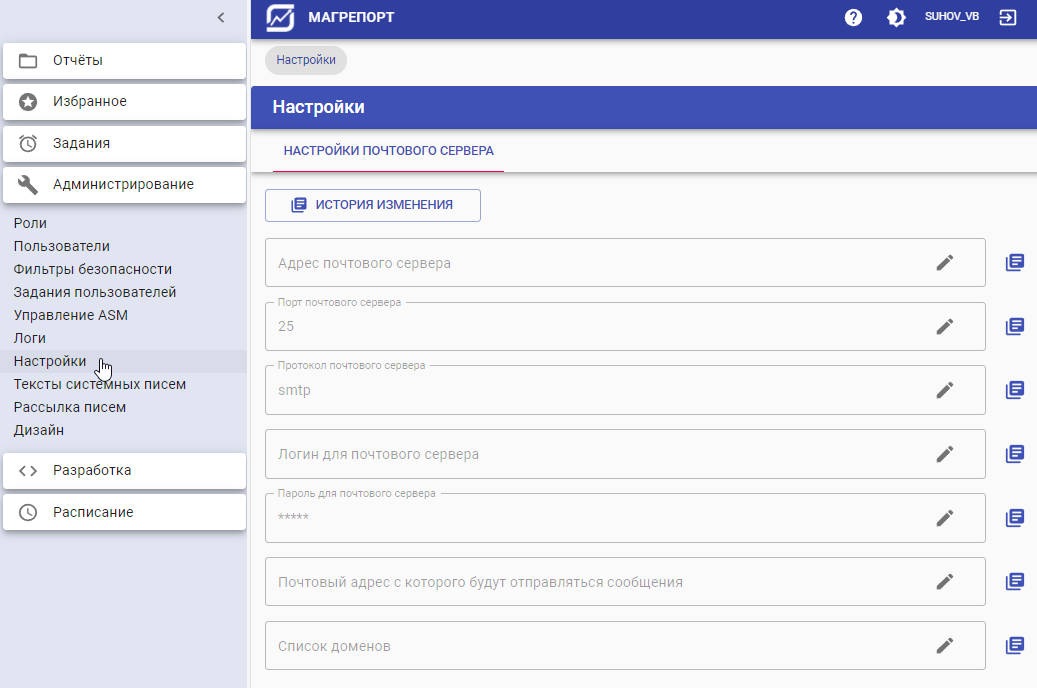
\includegraphics[width=\graphicswidth]{img/01-email-settings.png}
		\caption{Настройка параметров почтового сервера}
		\label{fig:email-settings}
	\end{figure}

	Значения параметров:
	\begin{itemize}
		\item \textit{Адрес почтового сервера} --- адрес хоста почтового сервера \\ (например: \textit{mail.example.com})
		
		\item \textit{Порт почтового сервера} --- порт, на котором работает почтовый сервер (по умолчанию: \textit{25})
		
		\item \textit{Протокол почтового сервера} --- в текущей версии системы поддерживается только \textit{smtp}
		
		\item \textit{Логин для почтового сервера} --- логин пользователя, от имени которого Магрепорт осуществляет авторизацию на почтовом сервере
		
		\item \textit{Пароль для почтового сервера} --- пароль для авторизации на почтовом сервере
		
		\item \textit{Почтовый адрес, с которого будут отправляться сообщения} --- почтовый адрес, подставляемый в графу <<От>> отправляемых писем
		
		\item \textit{Список доменов} --- список доменов, на которые разрешена отправка писем, если значение пусто --- отправка разрешена на любые домены
		
	\end{itemize}
	
	\subsection{Другие настройки} \label{subsection:other-settings}
	
	В разделе \textit{Maximum number of hierarchy levels} задаётся значение параметра ограничения на количество уровней вложенности каталогов:
	
	\begin{itemize}
		\item \textit{magreport.max-level-hierarchy} --- максимальное количество уровней вложенности каталогов объектов в Магрепорте (по умолчанию: \textit{128}), создать каталог, находящийся на большем уровне вложенности, не получится; параметр требуется для эффективной реализации внутренних алгоритмов системы
	\end{itemize}

	В разделе \textit{Admin mail address} задаётся значение почтового адреса администраторов сервера (для отправки уведомлений):
	
	\begin{itemize}
		\item \textit{mail.adminMailBox} --- электронный почтовый адрес администраторов сервера
	\end{itemize}	

	В разделе \textit{H2-console white list} задаётся список IP, с которых разрешён доступ в web-консоль репозитория H2

	\begin{itemize}
		\item \textit{magreport.h2.console.whitelist} --- список через запятую IP-адресов, с которых разрешён доступ в web-консоль репозитория H2 (https://<хост и порт Магрепорта>/h2-console), можно записывать в несколько строк, разделяя символом обратного слэша (<<$\backslash$>>)
	\end{itemize}	

	
	\section{Запуск и остановка системы}
	
	Для запуска системы Магрепорт требуется JRE версии 16. Запуск осуществляется командой:

	\begin{lstlisting}
		java -jar magreport.jar
	\end{lstlisting}
	
	При этом предполагается, что правильно сконфигурирована переменная окружения \textit{PATH}, либо в команде выше вместо \textit{java} явно указан путь к JRE версии 16. Магрепорт стартует HTTP-сервер, поэтому для успешного старта системы должны быть правильно сконфигурированы параметры HTTPS (см. пункт \ref{subsection:https-settings}), в каталоге, доступном на чтение пользователю, от имени которого выполняется Магрепогрт, размещён действующий сертификат сервера хоста, указанный в настройках порт должен быть свободен и разрешён к прослушиванию на сервере хоста. Также должно быть правильно сконфигурировано подключение к БД репозитория Магрепорт (см. пункт \ref{subsection:repository-settings}), если используется встроенный движок H2, то пользователю, от имени которого выполняется Магрепорт, должен быть доступен на редактирование каталог, в котором размещается БД. Также должен быть доступен на редактирование каталог, в котором размещаются файлы логов (см. пункт \ref{subsection:logging}). Если все эти условия выполнены, Магрепорт должен успешно запуститься и в стандартный поток вывода должно быть выведено диагностическое сообщение:
	
	\begin{lstlisting}
		Started MagReportBackendApplication
	\end{lstlisting}

	В промышленной среде рекомендуется запускать и останавливать систему как сервис, например, под управлением \textit{systemd}. В дистрибутивах Магрепорт для Linux предусмотрена регистрация соответствующего сервиса.
	
	Остановка системы осуществляется остановкой процесса приложения.
	
	\section{Обновление системы}\label{section:upgrade}
	
	При обновлении системы необходимо заменить файл magreport.jar свежей версией файла и добавить новые параметры в application.properties, если они появились в application.properties.template. Перед обновлением системы рекомендуется сделать резервное копирование БД репозитория (см. пункт \ref{section:backup}).
	
	\section{Резервное копирование}\label{section:backup}
	
	Для резервного копирования Магрепорта необходимо осуществлять резервное копирование БД репозитория. Если в качестве репозитория используется H2, необходимо делать резервную копию файлов \textit{db.mv.db} и \textit{db.trace.db} (если используется db в качестве имени базы, как задано в настройках по умолчанию) в каталоге размещения БД репозитория (по умолчанию ./db в домашнем каталоге Магрепорта).
	
	\section{Сервис мониторинга системных ресурсов}
	
	Сервис мониторинга системных ресурсов magreport-admin создан при помощи свободно-распространяемой библиотеки Spring Boot Admin и включен в дистрибутив системы Магрепорт. Сервис стартует отдельным java-процессом, выполняющим файл magreport-admin.jar. Исполняемый файл сервиса и соответствующий файл настроек application.properties расположены в каталоге magreport-admin домашнего каталога системы Магрепорт. По умолчанию сервис работает на 4443 порту и доступен по адресу:
	\begin{verbatim}
		https://имя-хоста-магрепорт:4443
	\end{verbatim}
	Вход в сервис осуществляется под учётной записью по умолчанию \textit{admin} с паролем \textit{admin}. Данные параметры могут быть изменены в application.properties. Также в application.properties необходимо указать хранилище сертификатов java в формате p12 и пароль к нему.
	
	Параметры application properties:
	
	\begin{itemize}
		\item \textit{server.ssl.key-store-type} --- тип хранилища сертификатов Java (должен быть PKCS12)
		\item \textit{server.ssl.key-store} --- файл хранилища сертификатов Java
		\item \textit{server.ssl.key-store-password} --- пароль хранилища сертификатов Java
		\item \textit{server.ssl.key-alias} --- алиас сертификата сервера в хранилище сертификатов Java
		\item \textit{server.port} --- порт сервиса
		\item \textit{spring.security.user.name} --- логин учётной записи (по умолчанию \textit{admin})
		\item \textit{spring.security.user.password} --- пароль учётной записи (по умолчанию \textit{admin})
	\end{itemize}
	
	Подробная документация по Spring Boot Admin может быть найдена здесь:
	
	\begin{center}
		\href{	https://codecentric.github.io/spring-boot-admin/2.5.1/}{	https://codecentric.github.io/spring-boot-admin/2.5.1/}
	\end{center}
	
\end{document}